\documentclass[presentation]{beamer}
\usetheme{CambridgeUS}
\usecolortheme{orchid}

\definecolor{themeColor}{HTML}{4e6eff}

\setbeamercolor*{structure}{bg=black,fg=themeColor}

\setbeamercolor*{palette primary}{use=structure,fg=white,bg=structure.fg}
\setbeamercolor*{palette secondary}{use=structure,fg=white,bg=structure.fg!75}
\setbeamercolor*{palette tertiary}{use=structure,fg=white,bg=structure.fg!50!black}
\setbeamercolor*{palette quaternary}{fg=white,bg=black}

\setbeamercolor{section in toc}{fg=black,bg=white}
\setbeamercolor{alerted text}{use=structure,fg=structure.fg!50!black!80!black}

\setbeamercolor{titlelike}{parent=palette primary,fg=structure.fg!50!black}
\setbeamercolor{frametitle}{bg=structure.fg!10!white,fg=structure.fg!50!black!80!black}

\setbeamercolor*{titlelike}{parent=palette primary}


\usepackage[utf8]{inputenc}
\usepackage{amssymb}
\usepackage{graphicx}
\usepackage{subfigure}
\usepackage{multirow}
\usepackage{hhline}
\usepackage{amsfonts,amstext,amssymb,wasysym}
\usepackage{fancyvrb}
\usepackage{alltt}
\usepackage{textcomp}
\usepackage{url}
\usepackage{multimedia,pgf}
\usepackage{geometry}
\usepackage{minted}
\usepackage{bibentry}
\usepackage{framed}
\usepackage{cleveref}
\nobibliography*

\title[04 - Continuous Integration]{\small{\input{../coursetitle}} \\
\normalsize{Continuous integration}}

% ! TeX root = 01-Introduction/01-Introduction.tex
\author[D. Pianini]{
Danilo Pianini\\
\texttt{{\footnotesize danilo.pianini@unibo.it}}}

\institute[UniBo]
{\textsc{Alma Mater Studiorum}---Universit\`a di Bologna}

\date[\today{}]{\input{../context} \\
\scriptsize \input{../date} - \input{../place} 
}

\pgfdeclareimage[height=0.625cm]{university-logo}{../images/logo}
\logo{\pgfuseimage{university-logo}}


\newcommand{\codefile}[4]{
	\begin{block}{\texttt{#2}}
		\inputminted[fontsize=#3,linenos=true,breaklines=true]{#4}{"workspace/#1/#2"}
	\end{block}
}

\begin{document}

\newcommand{\bashinline}[1]{\mintinline{bash}{#1}}

\AtBeginSubsection[]{%
  \begin{frame}<beamer>
    \frametitle{Outline}
    \tableofcontents[currentsection,currentsubsection]
  \end{frame}
  \addtocounter{framenumber}{-1}% If you don't want them to affect the slide number
}

%===============================================================================
\frame[label=coverpage]{\titlepage}
%===============================================================================

%===============================================================================
%===============================================================================
\section*{Outline}
%===============================================================================
%===============================================================================

\frame{\tableofcontents}

%===============================================================================
%===============================================================================

\section{Introduction}
\begin{frame}[fragile, allowframebreaks]{Why continuous?}
	\begin{block}{Avoid the integration hell}
		\begin{itemize}
			\item Work in parallel
			\item Don't waste developers' time with repetitive tasks
			\item Don't break stuff
		\end{itemize}
		Time is money
	\end{block}
	\begin{itemize}
		\item Software development used to take several months for ``integrating'' a couple of years of development \cite{fowlerci}
		\item Historically introduced by the extreme programming (XP) community
		\item Today used by companies that do not adopt XP
		\item IMVU \cite{imvu} delivers its software up to 50 times \textbf{per day}
		\item Google and Mozilla release \textbf{at least} once a day
	\end{itemize}
	\begin{block}{Higher frequency, lower risk \cite{semaphoreci}}
		
\includegraphics[width=.47\textwidth]{images/integration-traditional}
		~ \vline ~
		
\includegraphics[width=.47\textwidth]{images/integration-continuous}
	\end{block}
\end{frame}

\begin{frame}[fragile, allowframebreaks]{Improve over classic development}
	\begin{block}{Protoduction \cite{jargon}}
		\begin{center}
			
\includegraphics[width=.25\textwidth]{images/protoduction} \\
			When prototype code ends up in production
		\end{center}
		\begin{itemize}
			\item Classically used with a negative meaning
			\item Not so bad if done appropriately
		\end{itemize}
		\textbf{Make it easy to access and use the latest prototype}
	\end{block}
	\begin{block}{It's compiling \cite{xkcd303}}
		\centering
		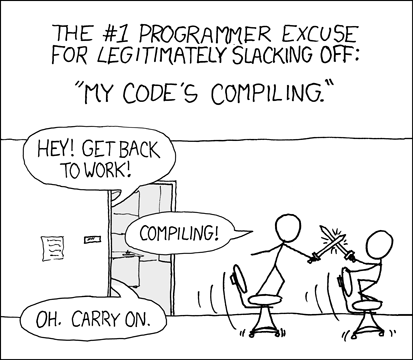
\includegraphics[width=.49\textwidth]{images/compiling}

		\textbf{Make the building process fast!} (or move it elsewhere...)
	\end{block}
\end{frame}

\begin{frame}[fragile]{Continuous Integration software}
	Software that promotes the practice of continuous integration
	\begin{itemize}
		\item Runs a build for every change in the project
		\item Prepares fresh environments where the builds are hosted
		\item Notifies the results, e.g. if a failure occurs
		\item Provides tools for deploying the produced artifacts
	\end{itemize}
	Hosted CI with free plans for open source projects are blossoming:
	\scriptsize
	\begin{itemize}
		\item Circle CI
		\item Codefresh
		\item Codeship
		\item drone.io
		\item Pipelines
		\item Travis CI
		\item Wercker
		\item ...
	\end{itemize}
\end{frame}

\section{Travis CI}

\begin{frame}[fragile]{Travis CI}
	\begin{itemize}
		\item Web based
		\item Well integrated with GitHub
		\begin{itemize}
			\item Build results are displayed in the repo without intervention
			\item Automatic build of any pull request
		\end{itemize}
		\item Free for open source projects
		\item Cronjobs
		\item Project-local configuration via YAML (in the \texttt{.travis.yml} file)
		\item Out of the box support for Gradle
		\item Dozens of deployment targets
	\end{itemize}
\end{frame}

\begin{frame}[fragile]{How it works}
	\begin{itemize}
		\item A web-hook can be registered to your GitHub repository that triggers Travis CI at each push
		\item Travis CI starts a pristine appropriate environment
		\begin{itemize}
			\item Can be a container or a full fledged virtual machine
		\end{itemize}
		\item The project gets cloned
		\item The configured commands are executed
		\item The configured deployments are performed
		\item If necessary, project managers are informed of the build status
	\end{itemize}
\end{frame}

\section{Configuration}

\subsection{Basics}

\begin{frame}{\texttt{.travis.yml}}
    \begin{itemize}
        \item Travis uses a project-local configuration
        \item A \texttt{.travis.yml} file \textit{must} be in your repository root
        \begin{itemize}
            \item of course, it must be tracked in git
        \end{itemize}
        \item It is a YAML file, very human-readable and easy to learn \footnote{\url{https://learnxinyminutes.com/docs/yaml/}} 
        \begin{itemize}
            \item Also it is a superset of JSON, so any valid JSON is a valid YAML
        \end{itemize}
        \item Supports basically any language that can get built on Linux or MacOS
        \begin{itemize}
            \item No support for Windows builds
        \end{itemize}
        \item Support for build matrix
        \begin{itemize}
            \item When your project can get built using different versions of different tools, you may want to test all of them
            \item It's a cartesian product of configurations
            \item Commit once, build on every supported environment
        \end{itemize}
    \end{itemize}
\end{frame}

\begin{frame}[fragile]{\texttt{.travis.yml}: the \texttt{language} section}
    \begin{itemize}
        \item Travis provides a number of default environments for the most common languages
        \begin{itemize}
            \item They differ by software installed by default
            \begin{itemize}
                \item e.g. the C\# compiler is not included if you run a Python build)
            \end{itemize}
            \item They behave differently
            \begin{itemize}
                \item e.g. if Java is specified as language, the system automatically searches for a \textit{build.gradle}, a \texttt{pom.xml} (Maven), or an Ant build script
            \end{itemize}
        \end{itemize}
        \item The first configuration required is a specification on which environment to work in
        \begin{itemize}
            \item Defaults to Ruby
        \end{itemize}
        \item For very simple projects, this might be enough of configuration
    \end{itemize}
    \begin{block}{Example}
        \begin{minted}{yaml}
language: python
        \end{minted}
    \end{block}
\end{frame}

\begin{frame}[fragile]{\texttt{.travis.yml}: custom behavior using the \texttt{script} section}
    \begin{itemize}
        \item The default configuration may be not suitable for you
        \begin{itemize}
            \item Either because you want to customize it
            \item Or because you are using something that is not in the spectrum of supported features
            \item Or because Travis does not use the right tool in the right way\footnote{\url{https://travis-ci.community/t/openjdk-12-no-longer-usable/2718}}
        \end{itemize}
        \item Bash commands can be configured to be executed in place of the default behavior
    \end{itemize}
    \begin{block}{Example}
        \begin{minted}[fontsize=\scriptsize]{yaml}
language: java
script:
  - cd myProject
  - ./gradlew runMyCustomTasks
  - cd ..
  - bash myPostBuildScript.sh
        \end{minted}
    \end{block}
\end{frame}

\begin{frame}[fragile]{\texttt{.travis.yml}: distribution selection in the \texttt{dist} section}
    \begin{itemize}
        \item By default, Travis CI builds in a Ubuntu Linux environment
        \item Ubuntu LTS is generally used
        \item The version of Ubuntu can be selected in a \texttt{dist} section
        \begin{itemize}
            \item At the time of writing, \texttt{trusty}, \texttt{xenial}, and \texttt{bionic} are \texttt{available}
        \end{itemize}
        \item Mac OS X can be used by specifying \texttt{os: osx} in place of \texttt{dist}
    \end{itemize}
    \begin{block}{Example}
        \begin{minted}[fontsize=\scriptsize]{yaml}
language: python
dist: trusty
script:
  - 'if [ "$TRAVIS_PULL_REQUEST" = "false" ]; then bash build.sh; fi'
  - 'if [ "$TRAVIS_PULL_REQUEST" != "false" ]; then bash build_pull_req.sh; fi'
        \end{minted}
    \end{block}
\end{frame}

\begin{frame}[fragile]{The build lifecycle in Travis}
    Every phase is a list of bash commands
    \begin{enumerate}
        \item Install --- Install any dependency required
        \begin{enumerate}
            \item \texttt{before\_install}
            \item \texttt{install}
            \item \texttt{before\_script}
            \item \texttt{script}
            \item \texttt{before\_cache}
            \item \texttt{after\_success} or \texttt{after\_failure} --- Execute additional scripts depending on the outcome of the build
            \item \texttt{before\_deploy}
            \item \texttt{deploy}
            \item \texttt{after\_deploy}
            \item \texttt{after\_script}
        \end{enumerate}
    \end{enumerate}
\end{frame}

\begin{frame}[fragile]{\texttt{.travis.yml}: Example with several phases}
    \begin{block}{Example}
        \begin{minted}[fontsize=\scriptsize]{yaml}
language: java
dist: bionic
before_install: echo Begin actual build
script:
  - ./gradlew clean build
  - ./gradlew buildDashboard
after_success: echo Build successful
after failure: sudo mail -s "Build failure" admin@company.org < /dev/null
before_deploy: echo Preparing for deploy
after_deploy: echo Deployment phase concluded.
        \end{minted}
    \end{block}
\end{frame}

\begin{frame}[allowframebreaks]{Build variables}
    Travis offers a number of environment variables that allow for fine tuning the build process.
    \begin{block}{\texttt{CI}, \texttt{TRAVIS}, \texttt{CONTINUOUS\_INTEGRATION}, and \texttt{HAS\_JOSH\_K\_SEAL\_OF\_APPROVAL}\footnote{Josh K. is a co-founder of Travis CI: \url{https://twitter.com/j2h}}}
        Always set to \texttt{true}. Used for detecting if the build is running on the Continuous integration environment
    \end{block}
    \begin{block}{\texttt{DEBIAN\_FRONTEND}}
        Always set to \texttt{noninteractive}. Some scripts use it to determine whether or not ask for user input.
    \end{block}
    \begin{block}{\texttt{USER}}
        Always set to \texttt{travis}. Do not depend on this value; do not override this value.
    \end{block}
    \begin{block}{\texttt{HOME}}
        Always set to \texttt{/home/travis}. Do not depend on this value; do not override this value.
    \end{block}
    \begin{block}{\texttt{LANG} and \texttt{LC\_ALL}}
        Always set to \texttt{en\_US.UTF-8}.
    \end{block}
    \begin{block}{\texttt{RAILS\_ENV}, \texttt{RACK\_ENV}, \texttt{MERB\_ENV}}
        Always set to \texttt{test}
    \end{block}
    \begin{block}{\texttt{JRUBY\_OPTS}}
         Always set to \texttt{"--server -Dcext.enabled=false -Xcompile.invokedynamic=false"}
    \end{block}
    \begin{block}{\texttt{JAVA\_HOME}}
        Set to the appropriate value, depends on the selected JDK
    \end{block}
    \begin{block}{\texttt{TRAVIS\_ALLOW\_FAILURE}}
        Set to \texttt{true} if the job is allowed to fail.
        Set to \texttt{false} if the job is not allowed to fail.
    \end{block}
    \begin{block}{\texttt{TRAVIS\_BRANCH}}
        For push builds, or builds not triggered by a pull request, this is the name of the branch.
        For builds triggered by a pull request this is the name of the branch targeted by the pull request.
        For builds triggered by a tag, this is the same as the name of the tag (\texttt{TRAVIS\_TAG}).
        Note that for tags, git does not store the branch from which a commit was tagged.
    \end{block}
    \begin{block}{\texttt{TRAVIS\_BUILD\_DIR}}
        The absolute path to the directory where the repository being built has been copied on the worker.
    \end{block}
    \begin{block}{\texttt{TRAVIS\_BUILD\_ID}}
        The id of the current build that Travis CI uses internally.
    \end{block}
    \begin{block}{\texttt{TRAVIS\_BUILD\_NUMBER}}
        The number of the current build (for example, \texttt{4}).
    \end{block}
    \begin{block}{\texttt{TRAVIS\_COMMIT}}
        The commit that the current build is testing.
    \end{block}
    \begin{block}{\texttt{TRAVIS\_COMMIT\_MESSAGE}}
        The commit subject and body, unwrapped.
    \end{block}
    \begin{block}{\texttt{TRAVIS\_COMMIT\_RANGE}}
        The range of commits that were included in the push or pull request. Note that this is empty for builds triggered by the initial commit of a new branch.
    \end{block}
    \begin{block}{\texttt{TRAVIS\_EVENT\_TYPE}}
        Indicates how the build was triggered. One of \texttt{push}, \texttt{pull\_request}, \texttt{api}, \texttt{cron}.
    \end{block}
    \begin{block}{\texttt{TRAVIS\_JOB\_ID}}
        The id of the current job that Travis CI uses internally.
    \end{block}
    \begin{block}{\texttt{TRAVIS\_JOB\_NUMBER}}
        The number of the current job (for example, \texttt{4.1}).
    \end{block}
    \begin{block}{\texttt{TRAVIS\_OS\_NAME}}
        On multi-OS builds, this value indicates the platform the job is running on. Values are \texttt{linux} and \texttt{osx} currently, to be extended in the future.
    \end{block}
    \begin{block}{\texttt{TRAVIS\_OSX\_IMAGE}}
        The osx\_image value configured in \texttt{.travis.yml}. If this is not set in \texttt{.travis.yml}, it is empty.
    \end{block}
    \begin{block}{\texttt{TRAVIS\_PULL\_REQUEST}}
        The pull request number if the current job is a pull request, \texttt{false} if it’s not a pull request.
    \end{block}
    \begin{block}{\texttt{TRAVIS\_PULL\_REQUEST\_BRANCH}}
        If the current job is a pull request, the name of the branch from which the PR originated.
        If the current job is a push build, this variable is empty.
    \end{block}
    \begin{block}{\texttt{TRAVIS\_PULL\_REQUEST\_SHA}}
        If the current job is a pull request, the commit SHA of the HEAD commit of the PR.
        If the current job is a push build, this variable is empty.
    \end{block}
    \begin{block}{\texttt{TRAVIS\_PULL\_REQUEST\_SLUG}}
        If the current job is a pull request, the slug (in the form \texttt{owner\_name/repo\_name}) of the repository from which the PR originated.
        If the current job is a push build, this variable is empty.
    \end{block}
    \begin{block}{\texttt{TRAVIS\_REPO\_SLUG}}
        The slug (in form: \texttt{owner\_name/repo\_name}) of the repository currently being built.
    \end{block}
    \begin{block}{\texttt{TRAVIS\_SECURE\_ENV\_VARS}}
        Set to \texttt{true} if there are any encrypted environment variables.
        Set to \texttt{false} if no encrypted environment variables are available.
    \end{block}
    \begin{block}{\texttt{TRAVIS\_SUDO}}
        \texttt{true} or \texttt{false} based on whether sudo is enabled.
    \end{block}
    \begin{block}{\texttt{TRAVIS\_TEST\_RESULT}}
        \texttt{0} if all commands in the script section (up to the point this environment variable is referenced) have exited with zero; \texttt{1} otherwise.
    \end{block}
    \begin{block}{\texttt{TRAVIS\_TAG}}
        If the current build is for a git tag, this variable is set to the tag's name.
    \end{block}
    \begin{block}{\texttt{TRAVIS\_BUILD\_STAGE\_NAME}}
        The build stage in capitalzed form, e.g. \texttt{Test} or \texttt{Deploy}. If a build does not use build stages, this variable is empty.
    \end{block}
\end{frame}

\subsection{Security}

\begin{frame}{Sensible data in builds}
    It could be useful to access private data from within a build
    \begin{itemize}
        \item Downloading a password-protected file
        \item Decrypt a password-encrypted file
        \item Open a keystore for signing a file
        \item Store an API key for a service used e.g. for testing
        \item Store a OAuth token for accessing a remote service
    \end{itemize}
    These data cannot be tracked on the repository (with the exception of encrypted files, but the problem is simply moved to passing the decrypt password to the build system).
    \begin{itemize}
        \item These data must be provided in form of enviroment variables
        \item Travis allows for inserting \textit{secure variables} in the web interface
    \end{itemize}
\end{frame}

\begin{frame}{Pull request attack}
    Usually, you want the integrator to build pull requests
    \begin{itemize}
        \item You want to test the integration before committing it
    \end{itemize}
    What if the pull request changes the \texttt{.travis.yml}, printing all the environment variables?
    \begin{itemize}
        \item The developer of an open source project is \textit{defenseless}
    \end{itemize}
    Travis CI does not allow access to secure variables when a pull request is executed
    \begin{itemize}
        \item As such, typically, the Travis build must be configured to detect whether a pull request is being bult, and in case don't perform tasks that depend on secure variables
    \end{itemize}
\end{frame}

\begin{frame}{Local Travis installation}
    Travis CI provides an installable module to help with several tasks otherwise tedious:
    \begin{itemize}
        \item Secure encryption of files
        \begin{itemize}
            \item You may need your private key for automatic signing, but you want it to be secret and only readable by builds you create
        \end{itemize}
        \item Secure encryption of global variables
        \begin{itemize}
            \item You may need your password or username or other sensible data to complete the deployment process, but you want it encrypted
            \item In case of OAuth tokens, you also don't want to waste time dealing with it manually.
        \end{itemize}
    \end{itemize}
    Install Travis CI locally:
    \begin{enumerate}
        \item Install RubyGems
        \begin{itemize}
            \item On Arch Linux: \texttt{pacman -Syu rubygems ruby-rdoc}
        \end{itemize}
        \item Issue: \texttt{gem install travis}
        \item Make sure your \texttt{PATH} includes the path where gems are installed
    \end{enumerate}
\end{frame}

\begin{frame}{Creating a secure variable}
    \begin{block}{From the web interface:}
        \begin{itemize}
            \item Go to the settings page
            \item Insert name and value
            \item Select if it should be displayed on the build
            \begin{itemize}
                \item Disable if the variable is meant to be secure
            \end{itemize}
            \item Use the environment variable in your build
        \end{itemize}
    \end{block}
    \begin{block}{From the local Travis CI application:}
        \begin{itemize}
            \item \texttt{travis encrypt MY\_SECRET\_ENV=super\_secret}
            \item The secured variable will be printed on terminal
            \item copy the \texttt{secure="..."} inside your \texttt{.travis.yml}
        \end{itemize}
    \end{block}
\end{frame}

\begin{frame}{Ecrypting a file}
    \begin{block}{From the local Travis CI application:}
        \begin{itemize}
            \item \texttt{travis encrypt-file my-super-secret-file}
            \item A new \texttt{my-super-secret-file.enc} file will be created
            \begin{itemize}
                \item It \textit{must} be added to track
            \end{itemize}
            \item The originating file \textit{must not} be in track, and must never have been (or it could be recovered): delete it immediately
            \item copy the \texttt{secure="..."} inside your \texttt{.travis.yml}
            \item Add the generated \texttt{openssl} command that appears on the terminal to the correct phase of your build
        \end{itemize}
    \end{block}
\end{frame}

\begin{frame}{Don't screw up: non-exhaustive list of advices}
    \begin{itemize}
        \item \textbf{DO} generate passwords, never use words related to the repository or project name
        \item \textbf{DON'T} use settings which duplicate commands to standard output, such as \bashinline{set -x} or \bashinline{set -v} in your bash scripts
        \item \textbf{DON'T} run \bashinline{env} or \bashinline{printenv}
        \item \textbf{DON'T} % ! TeX root = 04-ContinuousIntegration.tex
\bashinline{echo "$SECRET_KEY"}

        \item \textbf{DON'T} use tools that print secrets on error output, such as \texttt{php -i}
        \item \textbf{DOUBLE CHECK} before using git fetch or git push, as they might expose tokens or other secure variables
        \item \textbf{DOUBLE CHECK} for mistakes in string escaping
        \item \textbf{DOUBLE CHECK} before using settings that increase verbosity
        \item \textbf{PREFER} redirecting output to /dev/null when possible
        \begin{itemize}
            \item e.g. \bashinline{git push url-with-secret >/dev/null 2>&1}
        \end{itemize}
    \end{itemize}
\end{frame}

\subsection{Environment customization}

\begin{frame}[fragile]{Global variables}
    Further variables (besides those built-in) can be specified
    \begin{block}{Custom environment variables}
         \begin{minted}[fontsize=\normalsize]{yaml}
env:
  global:
    - FOO="bar"
    - BAR="baz"
        \end{minted}
    \end{block}
\end{frame}


\begin{frame}[fragile]{Operating system selection}
    Travis CI currently supports builds Linux, MacOS X, and Windows
    \begin{itemize}
        \item You can select the OS by using the \texttt{os} key
        \item \texttt{linux} is the default, if left unspecified
        \item \texttt{osx} and \texttt{windows} are the alternatives
        \item \texttt{dist} only makes sense under Linux, it is ignored otherwise
        \item Much like \texttt{dist}, the OSX version can be selected with \texttt{osx\_image}
        \item Under Windows, Git bash is used
    \end{itemize}
    \begin{block}{Using OSX}
         \begin{minted}[fontsize=\normalsize]{yaml}
os: osx
osx_image: xcode11
         \end{minted}
    \end{block}
    \begin{block}{Using Windows}
         \begin{minted}[fontsize=\normalsize]{yaml}
os: windows
         \end{minted}
    \end{block}
\end{frame}

\begin{frame}[fragile, allowframebreaks]{Installing packages}
    \begin{block}{Under Linux}
        Two options:
        \begin{enumerate}
            \item preferred: using the \texttt{addons} key
            \begin{minted}[fontsize=\scriptsize]{yaml}
addons:
  apt:
    # optional, updates the package database
    update: true
    packages:
    - graphviz
    - maven
            \end{minted}
        \item manually invoking apt-get
            \begin{minted}[fontsize=\scriptsize]{yaml}
before_install:
  - sudo apt-get update
  - sudo apt-get install -y graphviz maven
            \end{minted}
        \end{enumerate}
    Custom repositories can be configured
    \end{block}
    \begin{block}{Under MacOS X}
        Homebrew is supported:
        \begin{minted}[fontsize=\scriptsize]{yaml}
addons:
  homebrew:
    packages:
    - graphviz
    - maven
    update: true
        \end{minted}
        \begin{itemize}
            \item Falling back to the terminal is always possible
            \item Third party repositories (taps) are supported
            \item Brewfiles are supported
        \end{itemize}
    \end{block}
    \begin{block}{Under Windows}
        \begin{itemize}
            \item Direct installation via shell is the only way
            \item Much more limited than OSX and Linux
            \item Chocolatey\footnote{\url{https://chocolatey.org/}} is preinstalled
        \end{itemize}
        \begin{minted}[fontsize=\normalsize]{yaml}
    before_install:
        - choco install maven graphviz
        \end{minted}
    \end{block}
\end{frame}

\begin{frame}[fragile]{JDK limitations on Travis CI}
    \begin{block}{JDK on Travis}
        Travis allows to select the JDK with the \texttt{jdk} key.
        \begin{minted}[fontsize=\normalsize]{yaml}
jdk: openjdk11
        \end{minted}
        However (ab)uses \texttt{install-jdk.sh}\footnote{\url{https://github.com/sormuras/bach/blob/master/install-jdk.sh}} to do so:
        \begin{itemize}
            \item Unsupported on Windows
            \item Breaks very frequently (download locations change)
        \end{itemize}
    \end{block}
\end{frame}

\begin{frame}[fragile]{Working around limitations}
    \begin{itemize}
        \item A multiplatform Java installer exists: Jabba\footnote{\scriptsize\url{https://github.com/shyiko/jabba}}
        \item Jabba could be installed, then used to install and configure the JDK
        \item Installation is not trivial and requires some caveats
        \item I prepared a script to work around the issue\footnote{\scriptsize\url{https://github.com/DanySK/Gravis-CI/blob/master/.install-jdk-travis.sh}}
        \item Configures the JDK specified in the \texttt{JDK} environment variable
    \end{itemize}
    \begin{block}{}
        \begin{minted}[fontsize=\tiny]{yaml}
language: bash
os: windows
env:
    # This is a convenience variable for shortening download commands
    - GRAVIS="https://raw.githubusercontent.com/DanySK/Gravis-CI/master/"
    - JDK="adopt-openj9@1.11"
before_install:
  # Download the script
  - curl "${GRAVIS}.install-jdk-travis.sh" --output ~/.install-jdk-travis.sh
  # Download, install, configue the JDK, and export the configuration to the current shell
  - source ~/.install-jdk-travis.sh
        \end{minted}
    \end{block}
\end{frame}

\begin{frame}[fragile]{Git-sensitive versioning on Travis}
    \begin{itemize}
        \item In order to improve performance, by default Gradle limits the clone depth
        \begin{itemize}
            \item Namely, downloads only the latest 50 commits
            \item There is an option for that in git, we skipped it
        \end{itemize}
        \item This may impact the version computation!
    \end{itemize}
    \begin{block}{Clone the entire repository}
        \begin{minted}[fontsize=\normalsize]{yaml}
git:
  depth: false
        \end{minted}
    \end{block}
\end{frame}

\subsection{Deployment}

\begin{frame}[fragile]{GitHub Releases}
    Travis CI can automate deployment of artifacts on GitHub releases
    \begin{block}{Example \texttt{.travis.yml} configuration}
        \begin{minted}{yaml}
deploy:
  provider: releases
  api_key:
    secure: YOUR_API_KEY_ENCRYPTED
  file: "FILE TO UPLOAD"
  skip_cleanup: true
  on:
    tags: true
        \end{minted}
    \end{block}
    The authentication token for GitHub can be generated locally with:
    
    \texttt{travis setup releases}
    
    Remember to backup your travis file before running the command
\end{frame}

\begin{frame}[fragile]{surge.sh}
    A free host for static websites (HTML + Javascript)
    \begin{itemize}
        \item Install surge locally
        \item Create an account (with email and password)
        \item Create a new secret variable \texttt{SURGE\_LOGIN}
        \item Create a new secret variable \texttt{SURGE\_TOKEN}
        \begin{itemize}
            \item Obtain the value by using \bashinline{surge token}
        \end{itemize}
    \end{itemize}
    \begin{block}{Example \texttt{.travis.yml} configuration}
        \begin{minted}{yaml}
deploy:
  provider: surge
  project: ./build/docs/javadoc/
  domain: myjavadoc.surge.sh
  skip_cleanup: true
  on:
    all_branches: true
        \end{minted}
    \end{block}
\end{frame}

\begin{frame}[fragile]{Deploy to PyPI}
    The best place where to put your Python software modules!
    \begin{itemize}
        \item Sign up to PyPI
    \end{itemize}
    \begin{block}{Example \texttt{.travis.yml} configuration}
        \begin{minted}{yaml}
deploy:
  provider: pypi
  user: "Your (possibly encrypted) username"
  password:
    secure: "Your encrypted password"
        \end{minted}
    \end{block}
\end{frame}

\begin{frame}{Other targets}
anynines -- Appfog -- Atlas -- AWS CodeDeploy -- AWS Elastic Beanstalk -- AWS Lambda -- AWS OpsWorks -- AWS S3 -- Azure Web Apps -- bintray -- BitBalloon -- Bluemix CloudFoundry -- Boxfuse -- Catalyze -- Chef Supermarket -- Cloud 66 -- CloudFoundry -- Deis -- Engine Yard -- GitHub Pages -- Google App Engine -- Google Cloud Storage -- Google Firebase -- Hackage -- Heroku -- Launchpad -- Modulus -- npm -- OpenShift -- packagecloud.io -- Puppet -- Forge -- PyPI -- Rackspace Cloud Files -- RubyGems -- Scalingo -- Script -- TestFairy -- Ubuntu Snap Store -- Uploading Build Artifacts

\vspace{10pt}

Plus any target your build system can directly deal with (e.g. Maven Central)
\end{frame}

\subsection{Multi-OS and multi-environment}

\begin{frame}{The build matrix}
    \begin{itemize}
        \item Usually, software targets more than a platform
        \begin{itemize}
            \item e.g., support for Linux, Windows, and Mac OS
            \item Support for Java 8, 11, and 12
            \item Support for Amazon Corretto or other peculiar environments
        \end{itemize}
        \item You'd like to test it in all the supported configurations
        \begin{itemize}
            \item The example above would require 12 combinations
        \end{itemize}
        \item Gradle supports build matrices, building the cartesian product of:
        \begin{itemize}
            \item Non-global environment variables
            \item Operating systems
            \item Build environments
        \end{itemize}
    \end{itemize}
\end{frame}

\begin{frame}[fragile]{Build matrix example}
    \begin{block}{Expansion into four builds}
        \begin{minted}[fontsize=\scriptsize]{yaml}
# YAML anchors, allows for reusing variables, not Travis stuff
reference_jdk: &reference_jdk
  'JDK="adopt@1.11"'
reference_os: &reference_os
  'linux'
os:
  - osx
  - windows
  - *reference_os
env:
  # Not expanded
  global:
    - TERM=dumb
  # Expanded
  matrix:
    - *reference_jdk
    - JDK="adopt-openj9@1.11"
    - JDK="adopt@1.12"
    - JDK="adopt-openj9@1.12"
        \end{minted}
    \end{block}
\end{frame}

\begin{frame}[fragile]{Explicit inclusion and exclusion}
    \begin{block}{Expansion into four builds}
        \begin{minted}[fontsize=\scriptsize]{yaml}
os:
  - osx
  - windows
  - linux
env:
  matrix:
    - JDK="adopt-openj9@1.11"
    - JDK="adopt@1.12"
    - JDK="adopt-openj9@1.12"
matrix:
  exclude:
    - os: linux
      env: JDK="adopt@1.12"
  include:
    - os: linux
      env: JDK="adopt@1.8" LEGACY="true"
        \end{minted}
    \end{block}
\end{frame}

\begin{frame}{Build stages}
    \begin{block}{Problem: not all builds on a multi-build are equal}
        \begin{itemize}
            \item How to deploy only from a specific OS and environment?
            \item How to run different tests in different environments?
        \end{itemize}
    \end{block}
    Travis CI provides the concept of stages
    \begin{itemize}
        \item Groups of jobs that can be executed concurrently
        \item Multiple stages run sequentially
        \item A stage can start if all previous stage's builds completed successfully
        \item If no stage is mentioned, the default \texttt{test} is used
        \begin{itemize}
            \item Expanded builds from matrix are in \texttt{test}
        \end{itemize}
    \end{itemize}
    \begin{block}{Example}
        \begin{enumerate}
            \item Stage check: run all tests on the reference platform
            \item Stage multi-platform: run tests on all target platforms
            \item Stage deploy: publish artifacts
        \end{enumerate}
    \end{block}
\end{frame}

\begin{frame}[fragile, allowframebreaks]{Example with stages}
    \begin{block}{Matrix configuration and stage declaration}
        \begin{minted}[fontsize=\normalsize]{yaml}
os: [osx, windows, *reference_os]
stages: [check, test, deploy]
env:
  matrix:
    - *reference_jdk
    - JDK="adopt-openj9@1.11"
    - JDK="adopt@1.12"
    - JDK="adopt-openj9@1.12"
        \end{minted}
    \end{block}
    \begin{block}{Stage configuration}
        \begin{minted}[fontsize=\tiny]{yaml}
jobs:
  include:
    - stage: check
      name: "You can rename stages"
      os: *reference_os
      env: [*reference_jdk]
      script:
        - ./gradlew mySuperDeepCheck
    - stage: deploy
      name: "Reports and deployment"
      # Conditional execution
      if: repo = env(OFFICIAL_REPO_SLUG) AND type != pull_request
      os: *reference_os
      env: [PUBLISH="true", *reference_jdk]
      install:
        - bash install-my-dependencies.sh
      script:
        - ./gradlew buildArtifacts -x test
      after_success:
        - ./gradlew publish
        \end{minted}
    \end{block}
    \begin{block}{Selective deployment}
        \begin{minted}[fontsize=\normalsize]{yaml}
deploy:
  - provider: surge
    skip_cleanup: true
    project: "./build/myArtifact/"
    domain: mydomain.sh
    # Restrict deployment
    on:
      os: *reference_os
      repo: *official_repo
      branch: develop
      # Conditional deployments can check for a
      # *single condition* on an environment variable
      condition: $PUBLISH = "true"
        \end{minted}
    \end{block}
\end{frame}


% \begin{frame}{Workspaces}
% 
% \end{frame}

\subsection{Performance and issues}

\begin{frame}[fragile]{Caching}
    \begin{itemize}
        \item Builds may cache some information to be used on next runs
        \begin{itemize}
            \item Various dependencies
            \item e.g. maven and Gradle caches
        \end{itemize}
        \item Cached elements are packed in an archive
        \item The archive is downloaded and unpacked in subsequent builds
        \item There is one archive per OS per environment
        \item Minimal changes to the environment invalidate the cache
        \item Cache are not shared among the jobs of the same build
    \end{itemize}
    \begin{block}{}
        \begin{minted}[fontsize=\scriptsize]{yaml}
before_cache:
  # Cleanup the cache, for Gradle there are utilities in Gravis-CI
  - curl "${GRAVIS}.clean_gradle_cache.sh" --output .clean_gradle_cache.sh
  - bash .clean_gradle_cache.sh
cache:
  # Decide what to cache
  directories:
    - $HOME/.gradle/caches/
    - $HOME/.gradle/wrapper/
        \end{minted}
    \end{block}
\end{frame}

\begin{frame}[fragile, allowframebreaks]{Windows-specific issues}
    \begin{block}{Gradle daemon termination}
        \begin{itemize}
            \item Gradle builds on Windows won't terminate
            \item The Gradle wrapper remains alive
            \item The build is then forcibly killed 10 minutes after success by the system
        \end{itemize}
        \begin{minted}[fontsize=\footnotesize]{yaml}
install:
  - export GRADLE_OPTS="-Dorg.gradle.daemon=false $GRADLE_OPTS"
        \end{minted}
        \textbf{Note:} Gravis-CI JDK installation does it automatically
    \end{block}
    \begin{block}{Git autocrlf}
        \begin{itemize}
            \item Git by default converts LF line endings to CRLF on Windows
            \item This may disrupt code quality checks
            \item The repo must get deleted and recovered
        \end{itemize}
        \begin{minted}[fontsize=\footnotesize]{yaml}
before_install:
  - git config --global core.autocrlf false
  - git config core.autocrlf false
  - git rm --cached -r .
  - git reset --hard
        \end{minted}
    \end{block}
    \begin{block}{Windows defender}
        \begin{itemize}
            \item Windows has a default antivirus
            \item it kicks in often, slowing down the build
            \item Particularly slow if caches are used
            \item Delays build time significantly
            \item It's basically useless, and should be disabled
            \item Problem: it should be disabled before cache unpacking, but there is no stage available to fit commands in...
            \item Workaround: exploit command substitution on environment initialization
        \end{itemize}
        \begin{minted}[fontsize=\footnotesize,breaklines]{yaml}
env:
  global:
    # This work around disables it before caching
    - NO_WIN_DEFENDER=$(curl "${GRAVIS}.disable-windows-defender.sh" --output .no-defender.sh && source .no-defender.sh)
        \end{minted}
    \end{block}
\end{frame}

\subsection{Complete builds}

\begin{frame}[fragile]{Example with Python}
    \begin{itemize}
        \item The default Python environment uses isolated virtualenvs
        \item PyPy is supported out of the box
        \item The script entry is mandatory
        \item dependencies can be listed in a \texttt{requirements.txt} file
        \begin{itemize}
            \item Travis automatically runs \\
            \bashinline{pip install -r requirements.txt} ~\\
            during the install phase of the build
        \end{itemize}
    \end{itemize}
\end{frame}

\begin{frame}[fragile]{Java examples}
    Examples of rich, multi-project, multi-language, multi-target deployments are available at:
    \begin{itemize}
        \item \url{https://github.com/AlchemistSimulator/Alchemist}
        \item \url{https://github.com/Protelis/Protelis}
    \end{itemize}
\end{frame}

\section*{\refname}
%===============================================================================
\begin{frame}[allowframebreaks]
  \frametitle{\refname}
  \scriptsize
  \bibliographystyle{alpha}
  \bibliography{../bibliography}
\end{frame}
\section*{\refname}

\end{document}
